\documentclass[11pt,a4paper]{article}
\usepackage[T1]{fontenc}
\usepackage[utf8]{inputenc}
\usepackage{lmodern}
\usepackage[margin=2.5cm]{geometry}
\usepackage{amsmath,amssymb}
\usepackage{booktabs}
\usepackage{graphicx}
\usepackage[hidelinks]{hyperref}
\hypersetup{pdfauthor={Gianni Pilotti},pdftitle={Delta Hedging a Short SPY Straddle: Implied Against Realised Volatility},pdfcreator={},pdfproducer={}}
\setlength{\parindent}{0pt}
\setlength{\parskip}{6pt}

\title{Delta Hedging a Short SPY Straddle:\\Implied Against Realised Volatility}
\author{Gianni Pilotti}
\date{}

\begin{document}
\maketitle

\section{The Core Idea}
A short option that is delta hedged every day does not depend on where the market goes. It depends on one comparison: was the volatility it was sold at (implied) higher or lower than the volatility that actually happened (realised)?

The notebook tests this twice. First on simulated prices, where the true volatility is known. Then on real SPY data from 2010 to 2025, with VIX as the implied volatility.

\begin{itemize}
\item \textbf{Why it matters:} an option seller earns the volatility risk premium only if implied volatility exceeds realised volatility on average, and loses heavily when it does not.
\item \textbf{Why the input matters:} the real-data profit exists when the straddle is sold at the VIX level and disappears at a lower at-the-money level.
\end{itemize}

\section{Method}
\subsection{Price and delta}
European Black--Scholes with a dividend yield $q$. With $d_1=\dfrac{\ln(S/K)+(r-q+\tfrac12\sigma^2)T}{\sigma\sqrt T}$ and $d_2=d_1-\sigma\sqrt T$:
\[
C=Se^{-qT}N(d_1)-Ke^{-rT}N(d_2),\qquad
P=Ke^{-rT}N(-d_2)-Se^{-qT}N(-d_1).
\]
The straddle is $C+P$ at the same strike, and its delta is $e^{-qT}\left(N(d_1)+N(d_1)-1\right)$.

\subsection{The hedging engine}
The straddle is sold at the implied volatility $\sigma$ and hedged at the same $\sigma$. At each date the position holds $\Delta_i$ shares, the delta of the straddle. Between dates, cash earns the rate $r$ and the shares pay dividends. Every share trade costs a fraction $c$ of its value. At expiry the straddle payoff is paid and the shares held ($\Delta_{n-1}$) are sold:
\[
\text{P\&L}=\text{cash}_T+\Delta_{n-1}\,S_T-|S_T-K| .
\]
The result is the P\&L of the hedged position, reported as a percentage of the strike (spot at inception).

\subsection{Simulation and real data}
\begin{itemize}
\item \textbf{Simulation:} geometric Brownian motion, $S_0=100$, one-month ATM straddle ($T=21/252$), $r=3\%$, true volatility 20\%, 5,000 paths, seed 42. The straddle is sold at 20\% or 25\%, and hedged 1, 5, 21, 63 or 252 times. Costs are 0 or 0.1\% per trade.
\item \textbf{Real data:} every 21 trading days, sell a 21-day ATM straddle on SPY and hedge it daily at the close, 191 non-overlapping trades. $\sigma$ is VIX at the open times a scale (1.0 or 0.8). The rate is the 13-week T-bill (\verb|^IRX|), the dividend yield is the trailing 252-day dividends over spot, and the cost is 1 bp per share trade.
\item \textbf{Realised volatility:} standard deviation of the daily log returns over the trade, times $\sqrt{252}$.
\end{itemize}

\section{Results}
\textbf{Simulation.} Realised volatility is 20\%, and the price of the straddle at 25\% minus its price at 20\% is 1.149.

\begin{center}
\begin{tabular}{@{}rcccc@{}}
\toprule
 & \multicolumn{2}{c}{Sold at 20\%, no cost} & \multicolumn{2}{c}{Sold at 25\%, mean P\&L} \\
\cmidrule(lr){2-3}\cmidrule(lr){4-5}
Rebalances & Mean & Std & No cost & Cost 0.1\% \\
\midrule
1 & 0.026 & 3.510 & 1.177 & 1.172 \\
5 & $-0.034$ & 1.702 & 1.113 & 1.001 \\
21 & $-0.019$ & 0.858 & 1.129 & 0.871 \\
63 & $-0.002$ & 0.513 & 1.159 & 0.704 \\
252 & 0.006 & 0.261 & 1.166 & 0.256 \\
\bottomrule
\end{tabular}
\end{center}

\begin{itemize}
\item \textbf{True volatility:} when the straddle is sold at the true volatility, the hedged P\&L averages zero. Its standard deviation falls from 3.51 to 0.26 as the number of hedges goes from 1 to 252.
\item \textbf{Overpriced volatility:} sold at 25\% against 20\% realised, the seller keeps about 1.1 to 1.2, close to the price gap of 1.149, at every frequency.
\item \textbf{Costs:} with 0.1\% per trade, 252 rebalances cut the edge from 1.166 to 0.256.
\end{itemize}

\textbf{SPY, 2010 to 2025} (4,024 trading days, 191 trades):

\begin{center}
\begin{tabular}{@{}lcc@{}}
\toprule
 & Sold at VIX & Sold at $0.8\times$VIX \\
\midrule
Mean P\&L per trade (\% of spot) & $+0.79$ & $-0.03$ \\
Winning trades & 83\% & 62\% \\
Worst trade & $-7.5\%$ (10 Mar 2020) & $-8.2\%$ (10 Mar 2020) \\
\bottomrule
\end{tabular}
\end{center}
VIX averaged 18.4\% against 14.5\% realised. The correlation between trade P\&L and (implied variance $-$ realised variance) is 0.78 ($R^2=0.61$).

\begin{figure}[h]
\centering
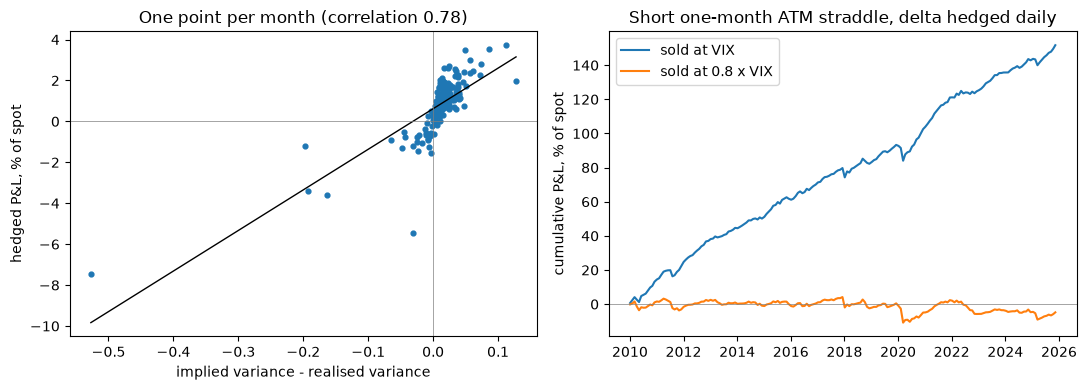
\includegraphics[width=0.95\textwidth]{../figures/spy_hedged_pnl.png}
\caption{Left: hedged P\&L against implied minus realised variance, one point per trade. Right: cumulative P\&L of the two runs.}
\end{figure}

\section{Worked Example}
\textbf{Premium and delta} (illustrative): $S=K=100$, $T=21/252$, $r=3\%$, $q=0$, $\sigma=20\%$.
\begin{align*}
C&=2.4271,\quad P=2.1774,\quad C+P=4.6045,\\
\Delta_{straddle}&=0.5288+(-0.4712)=0.0575,
\end{align*}
so the hedge holds 0.0575 shares per straddle sold. A quick check on the premium: an ATM straddle is worth about $0.8\,S\sigma\sqrt T=0.8\times100\times0.20\times\sqrt{21/252}=4.62$.

\textbf{Edge from overpriced volatility.} At $\sigma=25\%$ the premium is $5.7532$, so the gap is $5.7532-4.6045=1.1487$. The simulation mean (1.113 to 1.177 without costs) is close to this number.

\textbf{Is the edge real?} The $t$-statistic on the 191 trades is recomputed from the notebook's trade table. Sold at VIX: mean $0.794\%$, standard deviation $1.312\%$.
\begin{align*}
\text{s.e.}&=1.312/\sqrt{191}=1.312/13.82=0.0949,\\
t&=0.794/0.0949=8.37 .
\end{align*}
Sold at $0.8\times$VIX: mean $-0.025\%$, standard deviation $1.208\%$, so $t=-0.025/(1.208/13.82)=-0.29$. The average profit of the first run disappears when the ATM volatility is set 20\% below VIX.

\section{Limits}
\begin{itemize}
\item \textbf{No option prices:} implied volatility is approximated from VIX. The factor 0.8 is a judgement, not a measurement, and the conclusion depends on it.
\item \textbf{VIX is not ATM volatility:} VIX is a 30-day variance swap rate. With a negative skew it sits above the at-the-money volatility.
\item \textbf{Simplified market:} the bid-ask spread of the options is ignored, SPY options are priced as European, and the hedge uses closing prices only.
\item \textbf{Tail dominated:} the losses are concentrated in a few months when realised volatility jumped (March 2020). A sample of 191 trades holds few such events.
\item \textbf{Constant volatility in the simulation:} the simulated paths have no jumps and no volatility clustering, and real paths do. These are model outputs, not recommendations.
\end{itemize}

\end{document}
